
%Circular Loop  of Constant Current

\section{Circular Loop  of Constant Current}
\subsection{要求}
\noindent 画出不同半径均匀电流环方向图$l=\dfrac{\lambda}{20},\dfrac{\lambda}{6.28},\dfrac{\lambda}{2},0.61\lambda,\lambda,4\lambda$ 

\subsection{原理及推导}
均匀电流环的远场解


\begin{equation}
E_\phi\simeq \dfrac{ak\eta I_0e^{-jkr}}{2r} J_1\left( ka\sin\theta\right)
\end{equation}


\begin{equation}
H_\theta\simeq -\dfrac{E_\phi}{\eta}
\simeq -\dfrac{ak I_0e^{-jkr}}{2r} J_1\left( ka\sin\theta\right)
\end{equation}

由于, 最终需要得到归一化的功率方向图.所以常数项可以直接忽略. 
远场可以视为TEM波,故
\begin{equation}
P=\dfrac{E^2}{\eta} \simeq \left[J_1\left( ka\sin\theta\right)\right]^2
\end{equation}
编程时亦只关注这一部分. 


\subsection{结果与分析}
\subsubsection{方向图}
根据图\ref{fig:loopall}分析,有几个特殊的长度.

有一个长度书中没有提到,$a\simeq0.3\lambda$.一阶贝塞尔函数的第一个极大值约为3.9, 对应$ka\sin\theta=3.9$在$\theta=90^\circ$时,a约为0.3,此时$90^\circ$和$270^\circ$(平行于环的平面)方向第一次不再为主瓣方向. 
%在$a\le\lambda/6.28$时,可以认为方向图同Small Cirular Loop.在$a>\lambda/6.28$,不再可以认为是电小环. 必须考虑电流的空间分布带来的影响.

此时随着半径的增大,主瓣不再位于$90^\circ$和$270^\circ$(平行于环的平面)方向,而是向$0^\circ $和$180^\circ $移动. 当$a=0.61\lambda$时,$90^\circ$和$270^\circ$方向,恰好不再有辐射功率. 随着半径的继续增大,旁瓣增多的同时,其方向性也越来越好.

有一个特殊的尺寸当周长恰好为$\lambda$,即$a=\lambda/2\pi$,对于电流分布不均匀的环天线而言,其主辐射方向为$0^\circ $和$180^\circ $.
这里用CST做验证,如图\ref{fig:loopcst}.
\begin{figure}[!ht]
	\centering
	\includegraphics[width=12cm]{loop_all.eps}
	\caption{LoopPatterns} \label{fig:loopall}
\end{figure}

\begin{figure}[!ht]
	\centering
	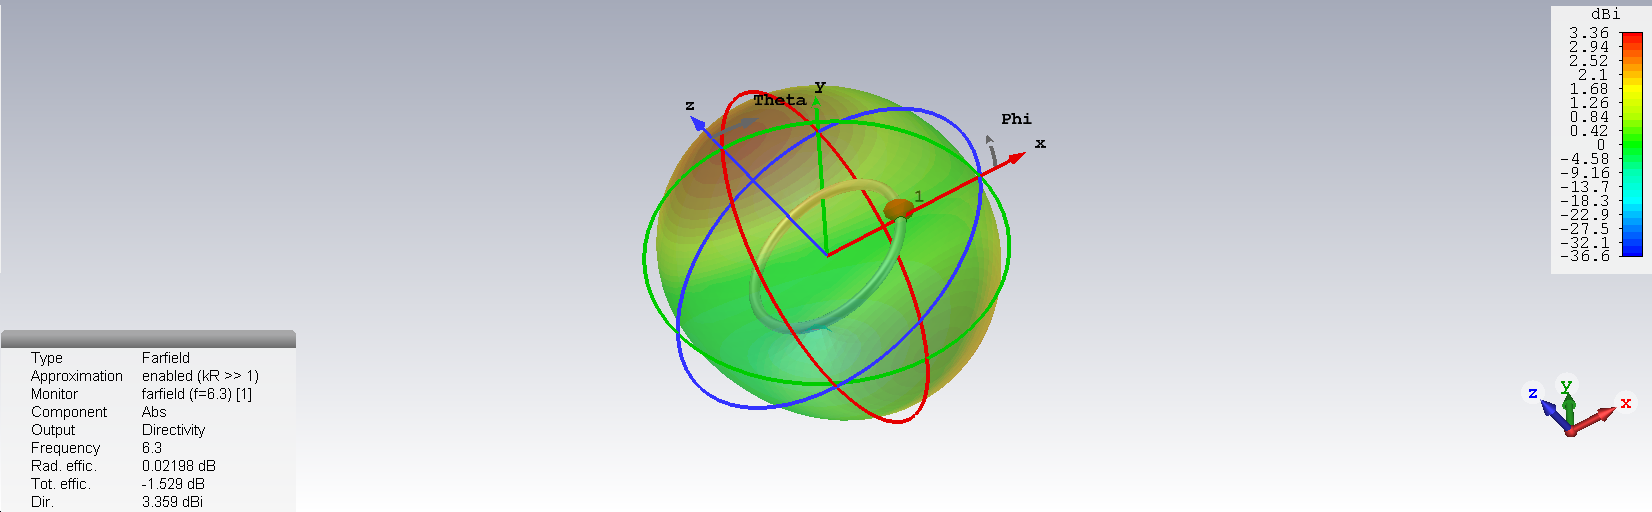
\includegraphics[width=12cm]{loop_cst.png}
	\caption{Pattern with CST} \label{fig:loopcst}
\end{figure}

\subsection{程序}
\noindent \textbf{绘制方向图主程序}
\begin{lstlisting}[language={matlab},keywordstyle=\color{blue!70},commentstyle=\color{red!50!green!50!blue!50},frame=shadowbox, rulesepcolor=\color{red!20!green!20!blue!20}] 
%主程序
clear
close all
A=[0.05,1/6.28,0.5,0.61,1,4];
%A=[0.15,0.2,0.85]
for i=1:length(A)
Fun_LoopPattern(A(i))
hold on
end
view(90,-90)
legend('\lambda/20','\lambda/6.28','\lambda/2',
'0.61\lambda','\lambda','4\lambda')
\end{lstlisting}
\noindent \textbf{子函数}
\begin{lstlisting}[language={matlab},keywordstyle=\color{blue!70},commentstyle=\color{red!50!green!50!blue!50},frame=shadowbox, rulesepcolor=\color{red!20!green!20!blue!20}] 
%子函数
function Fun_LoopPattern(A,StepNum)
if nargin<2
StepNum=2000;
end
theta=linspace(0,2*pi,StepNum);
x=2*pi*A*sin(theta);
U=(besselj(1,x)).^2;
U1=U/max(U);
polar(theta,U1);
end

\end{lstlisting}
